\documentclass{ctexbeamer}
\usetheme{Dresden}
\usecolortheme{spruce}
\usepackage{amsmath, amsfonts, amssymb}
\usepackage{tikz}
\usepackage{listings}
\usepackage{IEEEtrantools}
\special{dvipdfmx:config z 0} % delete this when release
\usetikzlibrary{positioning, arrows.meta, shapes.geometric}
\lstset{basicstyle=\ttfamily}

\title{Processor Arch: Pipelined}
\author{庄嘉毅}
\date{October 2022}

\def\QED{\hfill $\square$}
\def\st{\textrm{s.t.}\,}
\def\imply{\draw[-{Implies[]}, double distance=2pt]}
\DeclareMathOperator{\e}{e}
\newcommand{\ftitle}[1]{\frametitle{\hspace{4ex} {#1}}}
\newcommand{\bfig}[1]{
    \begin{figure}[hb]\centering\resizebox{\columnwidth}{!}{#1}
    \end{figure}
}
\newcommand{\roq}[1]{\rotatebox[origin=c]{-90}{#1}}

\usefonttheme{professionalfonts}
\everymath{\displaystyle}
\linespread{1.5}

\begin{document}

\begin{frame}
    \titlepage
\end{frame}

\section{为什么需要流水线?}
\begin{frame}
    \ftitle{为什么需要流水线?}

    \begin{itemize}
        \item 顺序结构无法发挥 CPU 的全部性能.
        \item 以五阶段处理器为例, 处理器在执行一个阶段时,
              其他阶段的电路都处于空闲状态.
    \end{itemize}

    \bfig{
        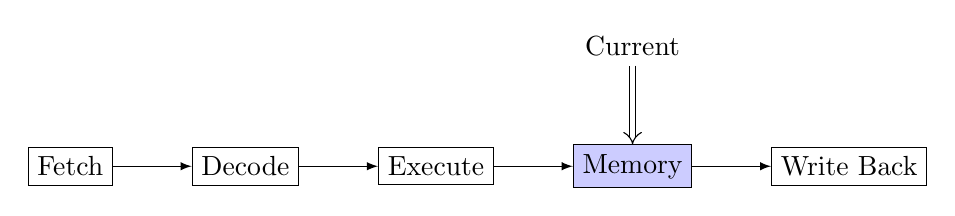
\begin{tikzpicture}
            \node [draw] (A) {Fetch};
            \node [draw, right=of A] (B) {Decode};
            \node [draw, right=of B] (C) {Execute};
            \node [draw, right=of C, fill=blue!20] (D) {Memory};
            \node [draw, right=of D] (E) {Write Back};
            \node [above=of D] (R) {Current};

            \draw[-latex] (A) -- (B);
            \draw[-latex] (B) -- (C);
            \draw[-latex] (C) -- (D);
            \draw[-latex] (D) -- (E);
            \imply (R) -- (D);
        \end{tikzpicture}
    }
\end{frame}

\begin{frame}
    \ftitle{理想的流水线复用}

    每个阶段的电路都在执行一条指令, 如同流水线一样依次进行.

    \bfig{
        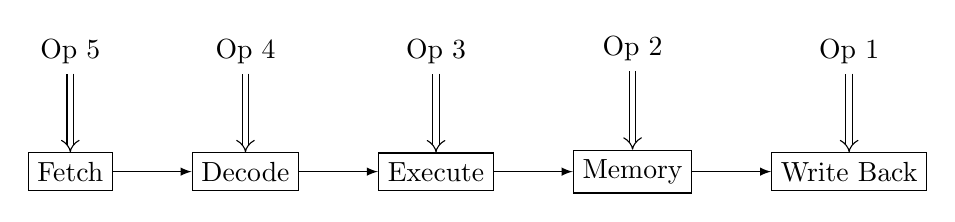
\begin{tikzpicture}
            \node [draw] (A) {Fetch};
            \node [draw, right=of A] (B) {Decode};
            \node [draw, right=of B] (C) {Execute};
            \node [draw, right=of C] (D) {Memory};
            \node [draw, right=of D] (E) {Write Back};
            \node [above=of A] (A1) {Op 5};
            \node [above=of B] (B1) {Op 4};
            \node [above=of C] (C1) {Op 3};
            \node [above=of D] (D1) {Op 2};
            \node [above=of E] (E1) {Op 1};

            \draw[-latex] (A) -- (B);
            \draw[-latex] (B) -- (C);
            \draw[-latex] (C) -- (D);
            \draw[-latex] (D) -- (E);
            \imply (A1) -- (A);
            \imply (B1) -- (B);
            \imply (C1) -- (C);
            \imply (D1) -- (D);
            \imply (E1) -- (E);
        \end{tikzpicture}
    }
\end{frame}

\section{流水线的实现}
\begin{frame}[fragile]
    \ftitle{改造顺序电路}

    \begin{itemize}
        \item 组合电路与代码不同, 其自身是没有时序保证的.
        \item 顺序电路的时序是如何保证的?
    \end{itemize}


    \begin{columns}
        \begin{column}{.5\linewidth}
            \bfig{
                \begin{tikzpicture}
                    \node (1) at (0, 1) {1};
                    \node (2) at (0, 0) {2};
                    \draw[black] (1, 1.5) rectangle (2, -0.5);
                    \node (ALU) at (1.5, 0.5) {ALU};
                    \draw (1) -- (1, 1);
                    \draw (2) -- (1, 0);
                    \node (3) at (3, 0.5) {3};
                    \draw (2, 0.5) -- (3);
                    \node (4) at (0, -1) {4};
                    \draw[black] (4, 1) rectangle (5, -1.5);
                    \node (ALU) at (4.5, -0.25) {ALU};
                    \draw (3) -- (4, 0.5);
                    \draw (4) -- (4, -1);
                    \node (7) at (6, -0.25) {7};
                    \draw (5, -0.25) -- (7);
                \end{tikzpicture}
            }            
        \end{column}
        \begin{column}{.5\linewidth}            
            \begin{lstlisting}
int a = 1 + 2;
int b = 4;
int c = a + b;
            \end{lstlisting}
        \end{column}
    \end{columns}
\end{frame}

\begin{frame}
    \ftitle{时序问题}
    \begin{itemize}
        \item 一个逻辑门的输出总是接到另一个逻辑门的输入端.
        \item 电信号传播需要时间, 但无法依赖于此来保证时序.
        \item 在组合逻辑计算完成之后, 如果输入不变, 其状态保持稳定.
        \item 在计算完成之前, 其状态是不稳定的, 不应该使用其结果.
        \item 需要有一个手段来保证稳态是能够对齐的.
    \end{itemize}
\end{frame}

\begin{frame}
    \ftitle{流水线寄存器}
    \begin{itemize}
        \item 寄存器的输出只有收到时钟信号才会改变, 能够起到状态对齐的作用.
        \item 为了在顺序处理器的五个状态之间创造明确的划分, 
            需要在每个状态之间加入寄存器.
    \end{itemize}

    \bfig{
        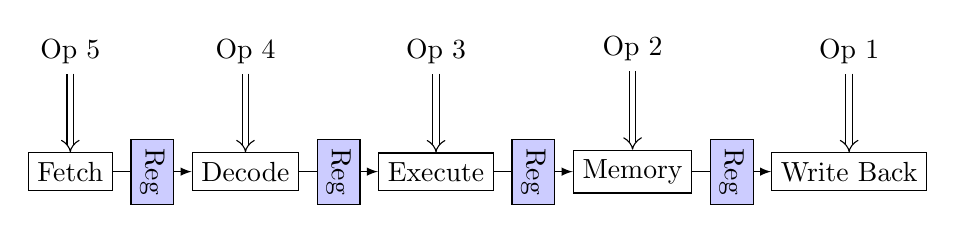
\begin{tikzpicture}
            \node [draw] (A) {Fetch};
            \node [draw, right=of A] (B) {Decode};
            \node [draw, right=of B] (C) {Execute};
            \node [draw, right=of C] (D) {Memory};
            \node [draw, right=of D] (E) {Write Back};
            \node [above=of A] (A1) {Op 5};
            \node [above=of B] (B1) {Op 4};
            \node [above=of C] (C1) {Op 3};
            \node [above=of D] (D1) {Op 2};
            \node [above=of E] (E1) {Op 1};

            \draw[-latex] (A) -- (B) node[midway, draw, fill=blue!20!white] {\roq{Reg}};
            \draw[-latex] (B) -- (C) node[midway, draw, fill=blue!20!white] {\roq{Reg}};
            \draw[-latex] (C) -- (D) node[midway, draw, fill=blue!20!white] {\roq{Reg}};
            \draw[-latex] (D) -- (E) node[midway, draw, fill=blue!20!white] {\roq{Reg}};
            \imply (A1) -- (A);
            \imply (B1) -- (B);
            \imply (C1) -- (C);
            \imply (D1) -- (D);
            \imply (E1) -- (E);
        \end{tikzpicture}
    }
\end{frame}

\end{document}
